\PassOptionsToPackage{table}{xcolor}
\documentclass[9pt,xcolor=x11names,compress]{beamer}

%% General document %%%%%%%%%%%%%%%%%%%%%%%%%%%%%%%%%%
\usepackage{graphicx}
\usepackage{tikz}
\usetikzlibrary{decorations.fractals,lindenmayersystems}
\usepackage{wasysym}
%%%%%%%%%%%%%%%%%%%%%%%%%%%%%%%%%%%%%%%%%%%%%%%%%%%%%%


%% Beamer Layout %%%%%%%%%%%%%%%%%%%%%%%%%%%%%%%%%%
\useoutertheme[subsection=false,shadow]{miniframes}
\useinnertheme{default}
\usefonttheme{serif}
\usepackage{palatino}

\setbeamerfont{title like}{shape=\scshape}
\setbeamerfont{frametitle}{shape=\scshape}

\setbeamercolor*{lower separation line head}{bg=DeepSkyBlue4} 
\setbeamercolor*{normal text}{fg=black,bg=white} 
\setbeamercolor*{alerted text}{fg=DeepSkyBlue4} 
\setbeamercolor*{example text}{fg=black} 
\setbeamercolor*{structure}{fg=black} 
 
\setbeamercolor*{palette tertiary}{fg=black,bg=black!10} 
\setbeamercolor*{palette quaternary}{fg=black,bg=black!10} 

\setbeamertemplate{blocks}[rounded][shadow=true]
\setbeamercolor{block title}{bg=DeepSkyBlue4}
\setbeamercolor{block title example}{bg=DeepSkyBlue4}
\setbeamercolor{block body}{bg=black!15!white}
\setbeamercolor{block body example}{bg=black!15!white}

\setbeamertemplate{navigation symbols}{}
%%%%%%%%%%%%%%%%%%%%%%%%%%%%%%%%%%%%%%%%%%%%%%%%%%

\author[Francisco Blanco-Silva]{Francisco Blanco-Silva}
\institute[USC]{University of South Carolina}
\date{
    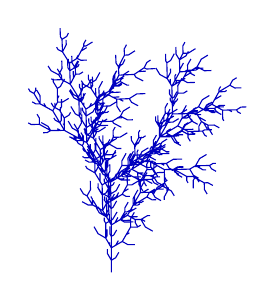
\begin{tikzpicture} 
    \draw [blue!75!black, rotate=90]
    [l-system={rule set={F -> FF-[-F+F]+[+F-F]}, axiom=F, order=4, step=2pt, 
        randomize step percent=25, angle=30, randomize angle percent=5}]
    lindenmayer system; 
    \end{tikzpicture}
    \\
}
\title{Lesson 4: Exponential Functions}

\begin{document}

\frame{\titlepage}

\section{What do we know?}
\subsection{}

\begin{frame}[t]
\frametitle{What do we know?}
\framesubtitle{The General Program}
\begin{columns}[t]
\begin{column}[t]{0.6\linewidth}
\begin{itemize}
\item Functions
\begin{itemize}
\item $x-$ and $y-$\alert{intercepts} ($f(x)=0$, $f(0)$)
\item \alert{Change} from $x=a$ to $x=b$ 
\begin{equation*}
    \Delta y = f(b)-f(a)
\end{equation*}
\item \alert{Average Rate of Change} from $x=a$ to $x=b$
\begin{equation*}
\text{ARC}=\frac{\Delta y}{\Delta x}=\frac{f(b)-f(a)}{b-a} 
\end{equation*}
\item \alert{Relative Rate of Change} from $x=a$ to $x=b$
\begin{equation*}
\text{RC} = \frac{\Delta y}{f(a)} = \frac{f(b) - f(a)}{f(a)}
\end{equation*}
\end{itemize}
\end{itemize}
\end{column}
\pause
\begin{column}[t]{0.4\linewidth}
\begin{itemize}
    \item Kinds of functions:
    \begin{itemize}
        \item \alert{Linear} \\ $f(x)=a + mx$
    \end{itemize}
\end{itemize}
\end{column}
\end{columns}
\end{frame}

\subsection{Warm-up}

\begin{frame}[t]\frametitle{Warm-up}
    
\framesubtitle{Exponential Rules}

\begin{block}{Exponential Rules}
Given $a, b > 0$, and any real values $x,y$:
\begin{itemize}[<+-|alert@+>]
    \item $a^{x+y} = a^x \cdot a^y$
    \item $a^{x-y} = \dfrac{a^x }{ a^y} $
    \item $a^{xy} = \big( a^x \big)^y = \big(a^y \big)^x$
    \item $(ab)^x = a^x \cdot b^x$
\end{itemize}
\end{block}

\uncover<5->{
\begin{example}
\begin{itemize}
    \item $\alert<6>{2^4 \uncover<6->{= 2 \cdot 2 \cdot 2 \cdot 2 = 16}}$
    \item $\alert<7>{5^{-3} \uncover<7->{= \dfrac{1}{5^3} = \dfrac{1}{125}}}$
    \item $\alert<8>{36^{1/2} \uncover<8->{= \sqrt{36} = 6}}$
    \item $\alert<9>{8^{5/3} \uncover<9->{= \big(8^{1/3}\big)^5 = 2^5 = 32}}$
    \item $\alert<10>{2^{1.56}}$
\end{itemize}
\end{example}
}
\end{frame}

\begin{frame}[c]\frametitle{Warm-up}
\framesubtitle{Exponential Rules}
\begin{center}
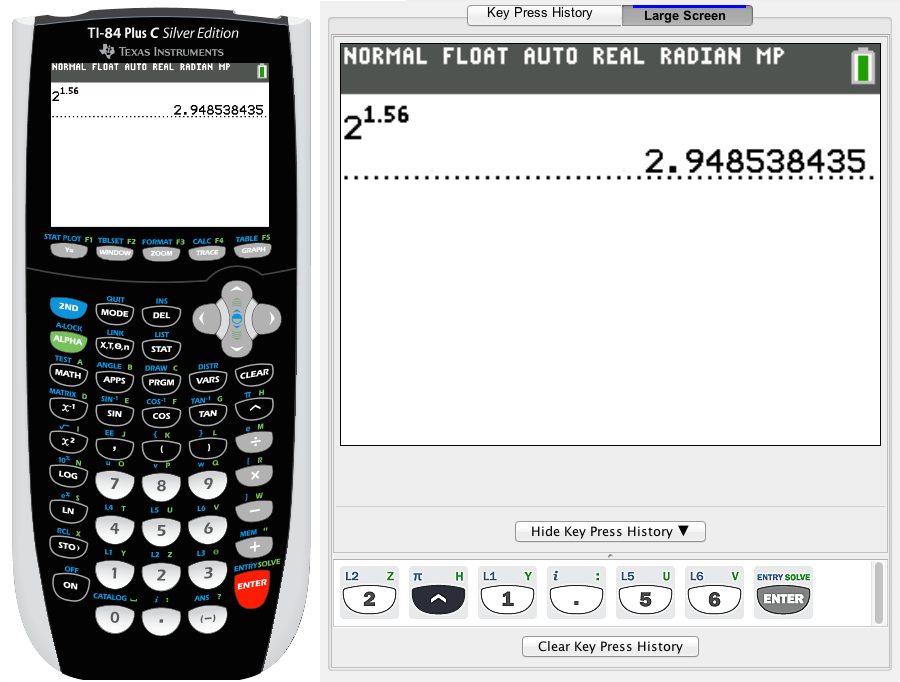
\includegraphics[width=0.9\linewidth]{ti84exponential.png}
\end{center}
\end{frame}

\begin{frame}[t]\frametitle{Warm-up}
    
\framesubtitle{Exponential Rules}
\begin{block}{Exponential Rules}
Given $a, b > 0$, and any real values $x,y$:
\begin{itemize}
    \item $a^{x+y} = a^x \cdot a^y$
    \item $a^{x-y} = \dfrac{a^x }{ a^y} $
    \item $a^{xy} = \big( a^x \big)^y = \big(a^y \big)^x$
    \item $(ab)^x = a^x \cdot b^x$
\end{itemize}
\end{block}

\begin{example}
\begin{itemize}
    \item $2^4 = 2 \cdot 2 \cdot 2 \cdot 2 = 16$
    \item $5^{-3} = \dfrac{1}{5^3} = \dfrac{1}{125}$
    \item $36^{1/2} = \sqrt{36} = 6$
    \item $8^{5/3} = \big(8^{1/3}\big)^5 = \big( \sqrt[3]{8} \big)^5 = 2^5 = 32$
    \item $\alert{2^{1.56} \approx 2.949}$
\end{itemize}
\end{example}
\end{frame}

\begin{frame}[c]\frametitle{Warm-up}
\framesubtitle{Exponential Rules}
\begin{example}[Solving (basic) exponential equations]
Solve for $a$ in the following equations:
\begin{itemize}
    \item \alert<2>{$a^3 = 125$}
    \begin{equation*}
        \uncover<2->{\alert<2>{a = 125^{1/3} = \sqrt[3]{125} = 5}}
    \end{equation*}
    \item \alert<3-4>{$27 a^3 = 8$}
    \begin{align*}
        \uncover<3->{\alert<3-4>{a^3} & \alert<3-4>{= \frac{8}{27}} &}
        \uncover<4->{\alert<4>{a} & \alert<4>{= \sqrt[3]{\frac{8}{27}} = \frac{2}{3}}}
    \end{align*}
    \item \alert<5->{$4.453a^{18} = 5.937$}
    \begin{align*}
        \uncover<5->{\alert<5->{a^{18}} & \alert<5->{= \frac{5.937}{4.453}} &}
        \uncover<6->{\alert<6->{a} &\alert<6->{= \bigg(\frac{5.937}{4.453}\bigg)^{1/18}}}
    \end{align*}
\end{itemize}
\end{example}
\end{frame}

\begin{frame}[c]\frametitle{Warm-up}
\framesubtitle{Exponential Rules}
\begin{center}
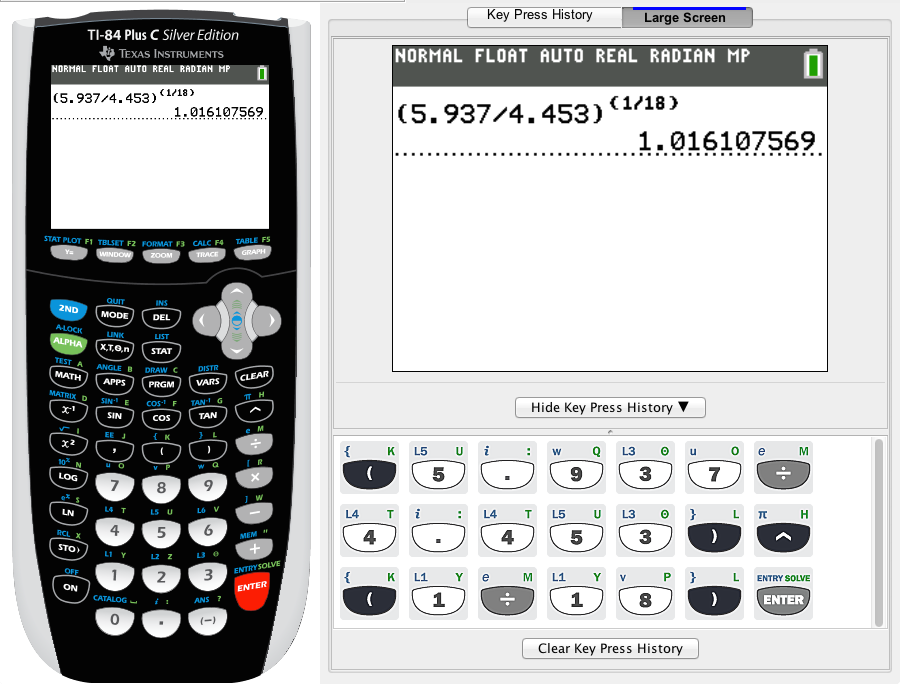
\includegraphics[width=0.9\linewidth]{ti84solveExp.png}
\end{center}
\end{frame}

\begin{frame}[c]\frametitle{Warm-up}
\framesubtitle{Exponential Rules}
\begin{example}[Solving (basic) exponential equations]
Solve for $a$ in the following equations:
\begin{itemize}
    \item $a^3 = 125$
    \begin{equation*}
        a = 125^{1/3} = \sqrt[3]{125} = 5
    \end{equation*}
    \item $27 a^3 = 8$
    \begin{align*}
        a^3 & = \frac{8}{27} &
        a & = \sqrt[3]{\frac{8}{27}} = \frac{2}{3}
    \end{align*}
    \item \alert{$4.453a^{18} = 5.937$}
    \begin{align*}
        \alert{a^{18}} & \alert{= \frac{5.937}{4.453}} &
        \alert{a} &\alert{= \bigg(\frac{5.937}{4.453}\bigg)^{1/18} \approx 1.016}
    \end{align*}
\end{itemize}
\end{example}
\end{frame}

\section{Exponential Functions}
\subsection{Definition}

\begin{frame}[t]
\frametitle{Exponential Functions}\framesubtitle{Definition}
We say that $P=P(t)$ is an \alert<1>{exponential function} with base $a$, if 
\begin{equation*}
   \alert<1>{P=P_0 a^t}
\end{equation*}
\pause
\begin{itemize}
    \item<2-> \alert<2>{$P_0$ is the initial quantity (when $t=0$)}
    \item<3-> \alert<3>{$a$ (the base) is the factor by which $P$ changes when $t$ increases by one unit.}
\end{itemize}
\pause\pause
If $a>1$ we say that $P$ models \alert<4>{exponential growth}.  If, on the other hand, $0<a<1$, we say that $P$ models \alert<4>{exponential decay}.

\pause
The base can be written as $a=1+r$, where $r$ is the decimal representation of the \emph{Relative Change}.  We also refer to $r$ in this case as the \alert<5>{growth/decay rate}. \pause  Note that
\begin{itemize}
    \item If $r>0$, we have exponential growth
    \item If $r<0$, we have exponential decay
\end{itemize}
\end{frame}

\subsection{Examples}
\begin{frame}
\frametitle{Exponential Functions}\framesubtitle{Examples}
\begin{example}
   Suppose that the initial amount of adrenaline in the blood is 15 mg.  Find a formula for the amount of adrenaline in the blood (in mg), $t$ minutes later if $A$ is:
   \begin{enumerate}
        \item \alert<2>{Increasing by 0.4 mg per minute}
        \item \alert<3>{Decreasing at a rate of 5\% a minute}
    \end{enumerate} 
\end{example}
\pause
\begin{enumerate}
    \item<2-> This indicates a linear increase, and 0.4 is the slope.  Since the initial amount must coincide with the $y-$intercept, the function is 
    \begin{equation*}
    A=f(t)=15+0.4t.
    \end{equation*}
    \item<3-> The percentage indicates we are dealing with exponential functions.  They give us $r=-0.05$, and the initial amount of 15 mg.  It must then be 
    \begin{equation*}
    A=f(t)=P_0 a^t \uncover<4->{= \overbrace{15}^{P_0} {\underbrace{(1-0.05)}_{a=1+r}}^t=15(0.95)^t.}
    \end{equation*}
\end{enumerate}
\end{frame}

\begin{frame}[t]
\frametitle{Exponential Functions}
\framesubtitle{Examples}
\begin{example}
40\% of an antibiotic is eliminated from the bloodstream every hour.  Find a function that expresses the amount of antibiotic in the blood after $t$ hours, assuming that the initial dose is 250 mg.  \alert<3>{Sketch the function and find the intercepts.}
\end{example}
\only<2>{% 
We are looking for $A=f(t)=A_0 (1+r)^t$, in mg.  The independent variable is $t$ in hours.  The initial dose is $A_0=250$, and the relative change is $r=-0.4$ (\alert{Why?}).  This gives us the function 
\begin{equation*}
    A=250(1-0.4)^t = 250 (0.6)^t
\end{equation*}}
\only<3>{%
\begin{center}
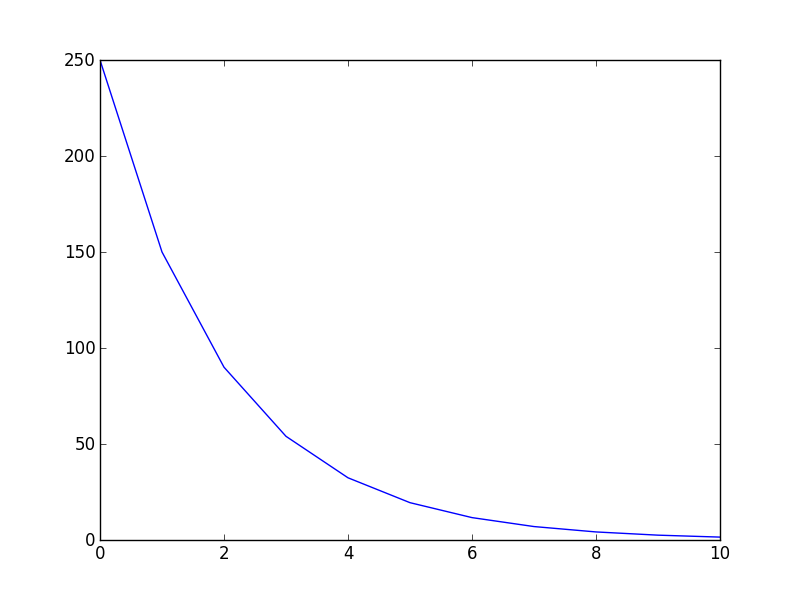
\includegraphics[width=0.65\linewidth]{figure_2.png}
\end{center}}
\end{frame}

\begin{frame}[c]\frametitle{Exponential Functions}
    
\framesubtitle{Examples}

\begin{center}
\only<1>{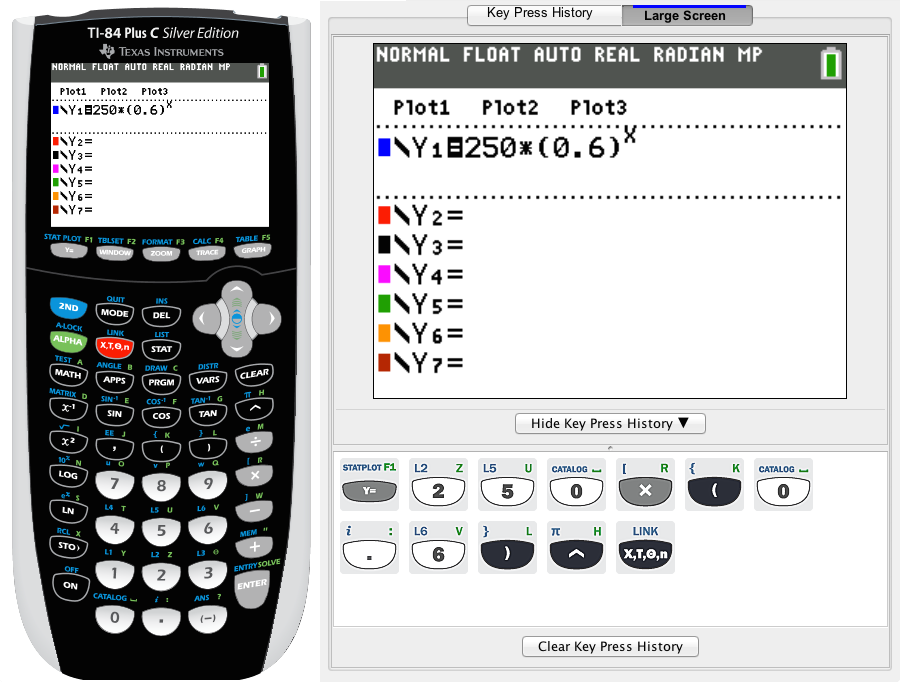
\includegraphics[width=0.9\linewidth]{ti84graph1.png}}
\only<2>{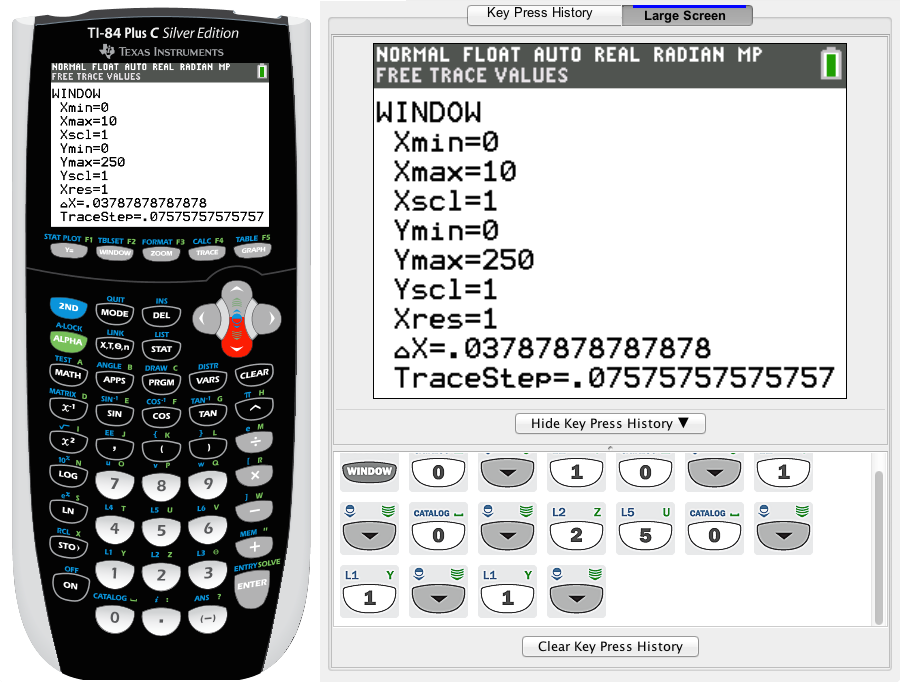
\includegraphics[width=0.9\linewidth]{ti84graph2.png}}
\only<3>{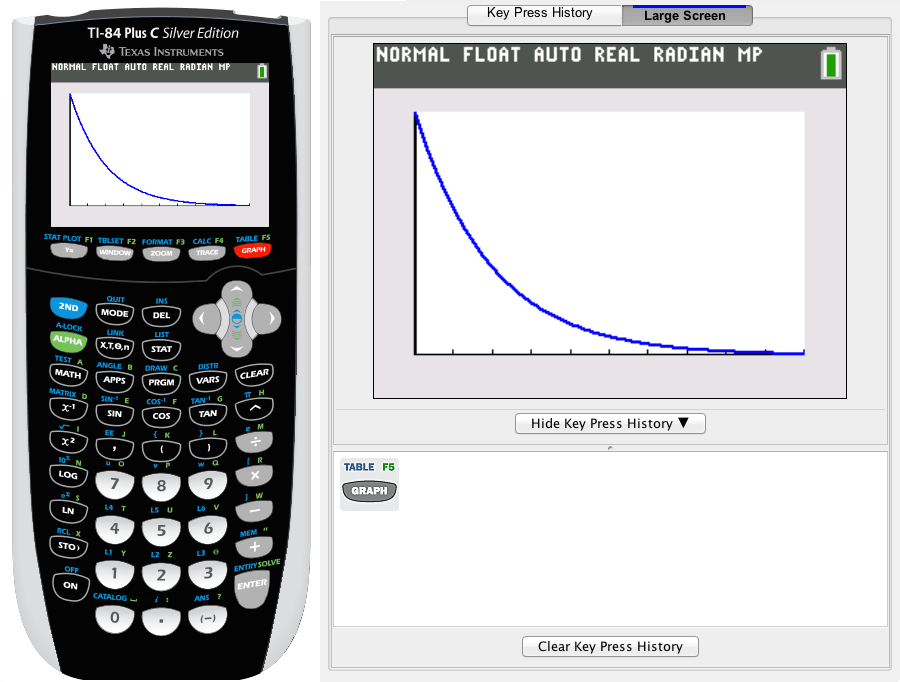
\includegraphics[width=0.9\linewidth]{ti84graph3.png}}
\end{center}

\end{frame}

\begin{frame}
\frametitle{Exponential Functions}
\framesubtitle{Examples}
\begin{example}
The following functions give the population of four different towns.  Time $t$ is expressed in years.        
\begin{itemize}
    \item $\displaystyle{\alert<2-3>{P=600(1.12)^t}}$
    \item $\displaystyle{\alert<4-5>{P=1000(1.03)^t}}$
    \item $\displaystyle{P=200(1.08)^t}$
    \item $\displaystyle{\alert<6->{P=900(0.90)^t}}$
\end{itemize}
Answer the following questions:
\begin{enumerate}
    \item \alert<2-3>{Which town has the largest growth rate?} \uncover<3->{\alert<3>{$r=0.12$, or an increase of 12\%}}
    \item \alert<4-5>{Which town has the largest initial population?} \uncover<5->{\alert<5>{$P_0 = 1000$}}
    \item \alert<6->{Are any of the towns decreasing in size?} \uncover<7->{\alert<7->{$r=-0.1$, or a decrease of 10\%}}
\end{enumerate}
\end{example}    
\end{frame}

\begin{frame}\frametitle{Exponential Functions}
   \framesubtitle{Examples}
   \begin{example}
    The population of the World increased from 4.453 billion in 1980 to 5.937 billion in 1998 and continued at the same percentage rate between 1998 and 2020.  Express the population (in billions) as a function of $t$ in years, and use it to compute the projected population in 2020.  
    \end{example}
    \pause
    \alert<2>{We search for a function of the form $P=P_0a^t$, with $t$ in years after 1980, and $P$ in billions.}  \pause \alert<3>{The initial value should then be $P_0=4.453$, and to find $a$ we use the other piece of information, $P(18)=5.937$.}
    \pause
    \alert<4>{%
    \begin{align*}
       4.453a^{18}&=5.937 &a=\Big( \frac{5.937}{4.453} \Big)^{1/18}\approx 1.016
    \end{align*}}
    \pause
    \alert<5>{It is then $P=4.453(1.016)^t$}

    \pause
    \alert<6>{The projected population in 2020 is $P(40)=4.453(1.016)^{40} \approx 8.402$ billion.}
\end{frame}

\end{document}